\begin{exercises}

\exercise 用一根线把一物体悬挂在升降机中。

(1) 当升降机以$ 3.0 $米/秒\textsuperscript{2}的加速度向上运动时,如果悬线的
张力是$ 10 $公斤,问此物的质量是多少?

(2) 当升降机以$ 3.0 $米/秒\textsuperscript{2}的加速度下降时,悬线的张力又
是多少?

\exercise 地球$ 24 $小时自转一周,地球半径为$  R = 6 3 7 8   $公里。一飞机
沿赤道自东向西飞行。以多大速度相对地球表面飞行时,飞机上
的东西的视重才正好等于实重?

\begin{wrapfigure}[8]{r}{11em}
    \centering
    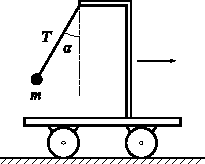
\includegraphics{figure/fig12.15}
    \caption{}
    \label{fig:12.15}
\end{wrapfigure}
\exercise 一质量为$ m $的小球用细线悬于
一架子上,架子固定在小车上,如图
\ref{fig:12.15} 所示。在下述诸情况下,求静
止平衡时线的方向(即图中$ \alpha $角)和线
中的张力$ T $。

(1) 小车沿水平面作匀速直线运动;

(2) 小车沿斜面作匀速直线运动,斜面倾角为$ \theta $;

(3) 小车以匀加速度$ a $沿水平直线运动;

(4) 小车自由地从倾角为$ \theta $的斜面上滑下;

(5) 用与斜面平行的加速度$ b $把小车沿斜面往上推,斜面倾
角为$ \theta $;

(6) 以同样大的加速度$ b $把小车从上述斜面上推下去。

\exercise 在以匀加速度$ a $沿平直轨道行驶着的车厢中,有一单摆,
摆长为$ l $,摆锤质量为$ m $,开始时用手拿住摆锤,使悬线保持竖
% 375.jpg
直且相对车厢为静止,然后突然放手,发生摆动。求:

(1) 悬线偏离竖直线$ \alpha $角时,摆锤的位能$ U $;

(2) 使摆锤偏离$ \alpha $角的力所作的功A;

(3) 悬线的最大偏离角$ \alpha _ { \text{max} } $;

(4) 证明$ \alpha _ { \text{max} } $是放手后摆相对于车厢静止平衡时摆线与竖直
线的夹角$  \alpha _ { 0 }   $的两倍。

\exercise 试用非惯性系中的牛顿力学方程解第三章中的例题7。

\exercise 一飞机以加速度$ \vec{a} $飞行,$ \vec{a} $与竖直向上方向的夹角为$\theta$,
驾驶员在地面上重为$ P $公斤。试求:

(1) 驾驶员作用在座位上的力为多少?

(2) 当$  \theta = 0   $时,情况如何?

(3) 当$ \theta = \dfrac { \uppi } { 2 }  $时,情况如何?

(4) 当$  \theta = \uppi, a = g   $时,情况如何?

(5) 当$  a = 0   $时,情况如何?

\exercise 一轰炸机以$ 1,000 $公里/时的速度俯冲后,即离开俯冲线
改沿一竖直圆周路线飞行,速率不变。若飞机在最低点的加速度
不得超过$ 4g $,求

(1) 竖直圆周的最小半径;

(2) 在圆周路径的最低点,一个$ 60 $公斤重的驾驶员的视重。

\exercise 一杂技演员表演飞车技木,骑一快速摩托车冲上圆柱形房
间的圆壁,沿着房间圆壁上的圆轨道快速行驶,车就不会掉下来。
试问:

(1) 设车与壁间的静摩擦系数为$  \mu _ { s }   $,房间半径为$ R $,若将车
与人整体视为一质点,$ v $至少为多大时,演员才不会掉下来?

(2) 设此房间的直径为$  D = 1 8 $米,车与人的重心离轮与壁接
触点的距离为$  h = 1 . 0   $米,$ \mu _ { s } = 0 . 4 $,$ v $至少为多大?

(3) 若车速$  v = 2 0   $米/秒,演员与水平面所成的角$\alpha$应为多
% 376.jpg
大?

\exercise 一圆环平放在水平面上,以匀角速度绕它的几何对称轴旋
转,圆周上的速度为$ v $,证明环中的胁强(即应力)为$  \rho v ^ { 2 } / g   $。$\rho$是
单位长度圆环的质量,$ g $是重力加速度。

\exercise 试用非惯性系的牛顿力学方程解第三章的习题27。

\exercise 一炮弹沿水平弹道(可近似看成直线)以$ 900 $米/秒的速度
飞行,炮弹是在北纬$ 60^\circ $向着正北方向距离$ 18 $公里处的目标发射
的。若不考虑地球的公转,略去空气阻力,不计惯性离心力,问
因地球自转,炮弹打到目标附近时,在水平方向偏离多少?偏向
什么方向?

\exercise 一半径为$ R $的水平大圆盘绕通过圆心的竖直线旋转,角
速度为$\omega$。试问:

(1) 站在圆盘中心的人用手枪射击盘边缘上一点$ B $,子弹
速度为$ v $,问直接对准$ B $射击能否射中?若不能应给什么样的提
前量$\wideparen{AB}$,才能击中$  B $?

(2)如果人站在盘边缘$ C $处射击$ B $,$ BC $为直径,他应当怎样
瞄准?

\exercise 在北纬$  4 0 ^ { \circ }   $,一质量为$ 60 $公斤的人向东以$ 9.0 $米/秒的速
度跑步,求他所受的科里奥利力。

\exercise 图\ref{fig:12.13}中$ A, B $两质点间的相对加速度称为潮汐加速度。
试求地面上相距为$ 10 $厘米的两质点之间的潮汐加速度$ a $。
% 377.jpg

\end{exercises}